\chapter{Architectural Design}

\section{Overview}

At the highest level of abstraction, the architecture of Data4Help and AutomatedSOS system is a common three-tier client/server paradigm, as shown in Figure \ref{f:3tier}.





\begin{figure}[H]
\centering
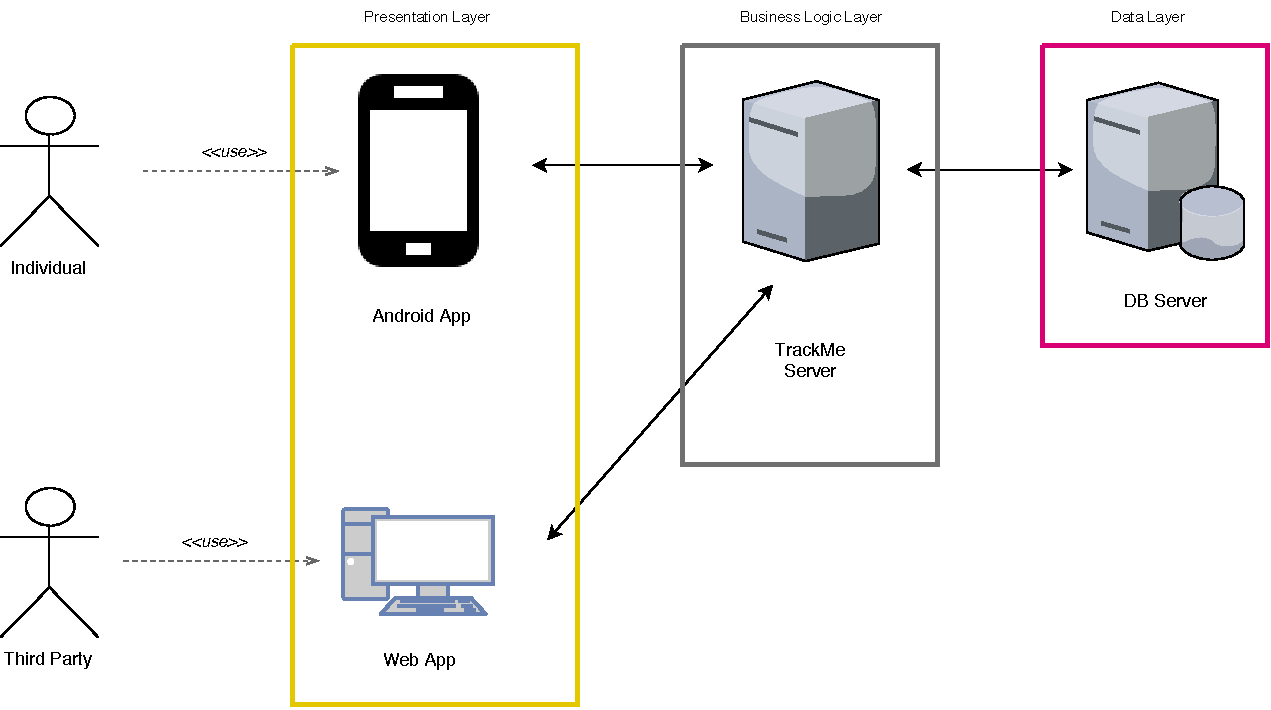
\includegraphics[scale=0.65]{resources/overview}
\caption{The 3 tier architecture of the system}\label{f:3tier}
\end{figure}
\noindent
The three layers are the following:

\begin{itemize}
\item \textbf{Presentation layer}: this layer is hosted on the users' devices, that are the smartphone for the individuals and a computer with a browser for third parties.
The GUIs are deployed in this layer.
\item \textbf{Business logic layer}: this layer contains the main components of the systems that carry out the operations needed for Data4Help and AutomatedSOS services.
\item \textbf{Data layer}: this layer is responsible for managing all the data of the system. 
In particular, it stores the data on persistent devices and makes them available when requested by the TrackMe servers.
\end{itemize}
The structure displayed in Figure \ref{f:3tier} is not to be understood as a rigid constraint on the implementation choices, but it represents where most of the three three logic layers are deployed.
For examples, it is possible that part of the data is (temporarily) stored on the clients in order to reduce latency or that some presentation logic is deployed on the TrackMe Server in order to achieve a more dynamic GUI.





\section{Component view}
The diagram in Figure \ref{f:comp_diag} examines in more detail the subcomponents composing the TrackMe server.
Some components requires external services, this is shown by means of pending required interfaces.
All the four components defined below have access to the database server interface in order to store and retrieve the data necessary for their correct operation.

\begin{figure}[H]
\centering
\includegraphics[width=\linewidth]{resources/uml/compdiag}
\caption{Component Diagram}\label{f:comp_diag}
\end{figure}

\noindent
As shown, there are four main components in the business logic server:

\begin{itemize}
\item \textit{Login Manager}: is responsible for the login and registration of the users, both individuals and third parties.
\item \textit{Data Collector}: is responsible of collecting data from the Android App. 
It also forwards the proper data to the Automated SOS component.

\item \textit{Data Manager}: receives and handles requests from third parties and push to them new data when available and the subscription is valid.
For certain functionalities, for example for geographically filter the data, the Data Manager component requires an external API to a map service.
It also makes possible for the individuals to visualize their data.

\item \textit{Automated SOS}: handles the subscriptions for the SOS service. 
Every time that it receives new data from the Data Collector, the component checks whether the thresholds are crossed, in this case it immediately calls an ambulance through an external API.
\end{itemize}
In addition, Figure \ref{f:comp_diag} shows that the Android App component requires an interface towards the wearable device, from which it will gather the eHealth Data.




\section{Deployment view}



The diagram in Figure \ref{f:depl_diag} shows the physical deployment of system's artifacts on various nodes.
In particular, the nodes are:

\begin{itemize}
\item \textit{Smartphone}: this device is used by an individual, then the Android Application is deployed here. This node interacts with the Business Server.
\item \textit{Personal Computer}: this device is used by a third party, only a modern browser compatible with HTML5 and CSS3 is required. Actually, there are no artifacts of our system deployed on this node, because the interaction is carried out with a Web App directly towards the Business Server.
\item \textit{Business Server}: this is the core node of our system.
All the Business Logic is deployed here, possibly by means of an Application Server like GlassFish.
This is the only node that interact with the Database node.
\item \textit{Data Server}: on this node are deployed all the artifacts necessary to manage the data.
\end{itemize}


\begin{figure}[h]
\centering
\includegraphics[width=\linewidth]{resources/uml/depldiag}
\caption{Deployment Diagram}\label{f:depl_diag}
\end{figure}

\section{Component Interfaces}
The following diagram explicits what features each component must provide to guarantee the correct functioning of Data4Help features, highliting the dependencies among the various components.
To make the diagram more clear, the crossing arrows have different colours and the interfaces interacting with external components are highlited in orange.

\begin{figure}[h]
\centering
\includegraphics[width=\linewidth]{resources/uml/Interfacediag}
\caption{Interface Diagram}\label{f:inter_diag}
\end{figure}

Here is presented a brief description of the functionalities provided by each operation:
\begin{itemize}
\item Application
\begin{itemize}
\item \textbf{forwardAccessRequest}: forwards the third party data access request to the individual's application. The data request is taken as an input parameter because it is needed to retrieve all the information about the request: who is the requester, in which data he is interested in.
\end{itemize}
\item Wearable Service
\begin{itemize}
\item \textbf{downloadData}: downloads to the application the data stored in the wearable.
\item \textbf{checkVitalSensors}: checks if the wearable is capable of measuring at least one vital parameter, either the blood pressure or the heart rate.
\end{itemize}
\item WebApplication
\begin{itemize}
\item \textbf{notifyEndSubscription}: notifies the third party about an ended data subscription in an asynchronous way. The data request is taken as an input in order to 
\item \textbf{sendData}: sends the given data to the webApplication.
\end{itemize}
\item DataCollector
\begin{itemize}
\item \textbf{sendData}: sends the gathered data from the app to the data collector.
\end{itemize}
\item MapService
\begin{itemize}
\item \textbf{retrieveMapAreas}: search the city name bound to the coordinates received.
\end{itemize}
\item DataManagerService
\begin{itemize}
\item \textbf{checkPrivacyCostraints}: scan the input data and checks if the number of i
\item \textbf{giveAccess}: allows the individual data gathering from the given third party request to be processed.
\item \textbf{denyAccess}: denies the individual data gathering from the given third party request to be processed.
\item \textbf{subscribeData}: activates the data subscription of the given data request.
\end{itemize}
\item LoginService
\begin{itemize}
\item \textbf{createAccount}: uses the given credentials to create a Data4Help account.
\item \textbf{logIn}: allows users to access to Data4Help through their username (or tax code) and password.
\end{itemize}
\item AutomatedSOS
\begin{itemize}
\item \textbf{subscribe}: activates the AutomatedSOS service for the individual associated to the given tax code.
\item \textbf{unsubscribe}: stops the AutomatedSOS for the individual associated to the given tax code.
\item \textbf{checkVitalThresholds}: checks if the data of the vital paramaters have crossed the critical thresholds
\end{itemize}
\item AmbulanceService
\begin{itemize}
\item \textbf{callAmbulance}: calls an ambulance, using the input coordinates to specify the destination.
\end{itemize}
\item DBMS
\begin{itemize}
\item \textbf{addSubscriber}: adds in the database the individual associated to the tax code as an AutomatedSOS subscriber
\item \textbf{removeSubscriber}: remove the AutomatedSOS subscriber associated to the tax code from the database.
\item \textbf{getData}: use the given data filters to build the respective query for the database, in order to access the desired data.
\item \textbf{uploadData}: adds the given data and the associated geographical position to the database.
\item \textbf{retrieveAccount}: checks if the given credentials are in the database.
\item \textbf{createAccount}: adds a new user account to the database using the given credentials.
\item \textbf{checkDuplicate}: checks if the given username or tax code are already inserted in the database.
\end{itemize}
\end{itemize}



\section{Runtime view}
\subsection{User registration}
\begin{figure}[h]
\centering
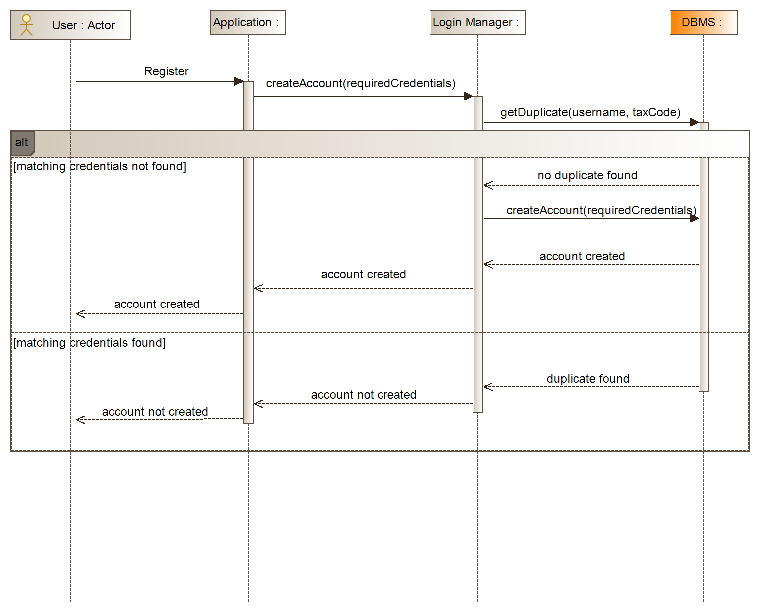
\includegraphics[width=\linewidth]{resources/uml/sequence/Registration.png}
\end{figure}

\subsection{User log in}
\begin{figure}[h]
\centering
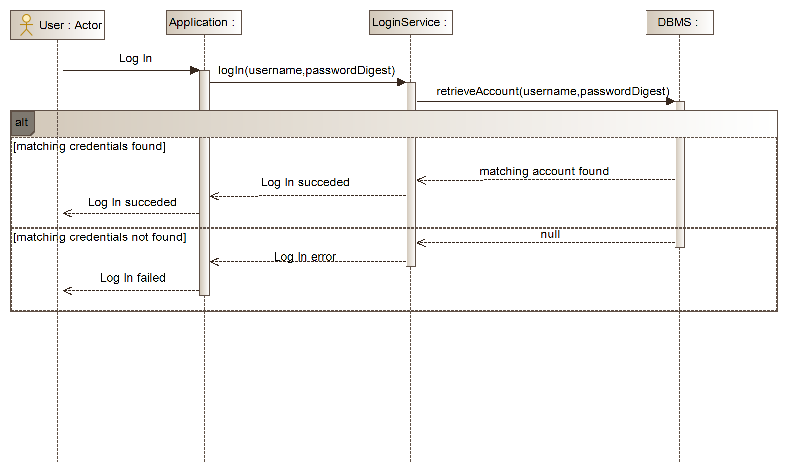
\includegraphics[width=\linewidth]{resources/uml/sequence/LogIn.png}
\end{figure}

\subsection{Individual data upload}
\begin{figure}[h]
\centering
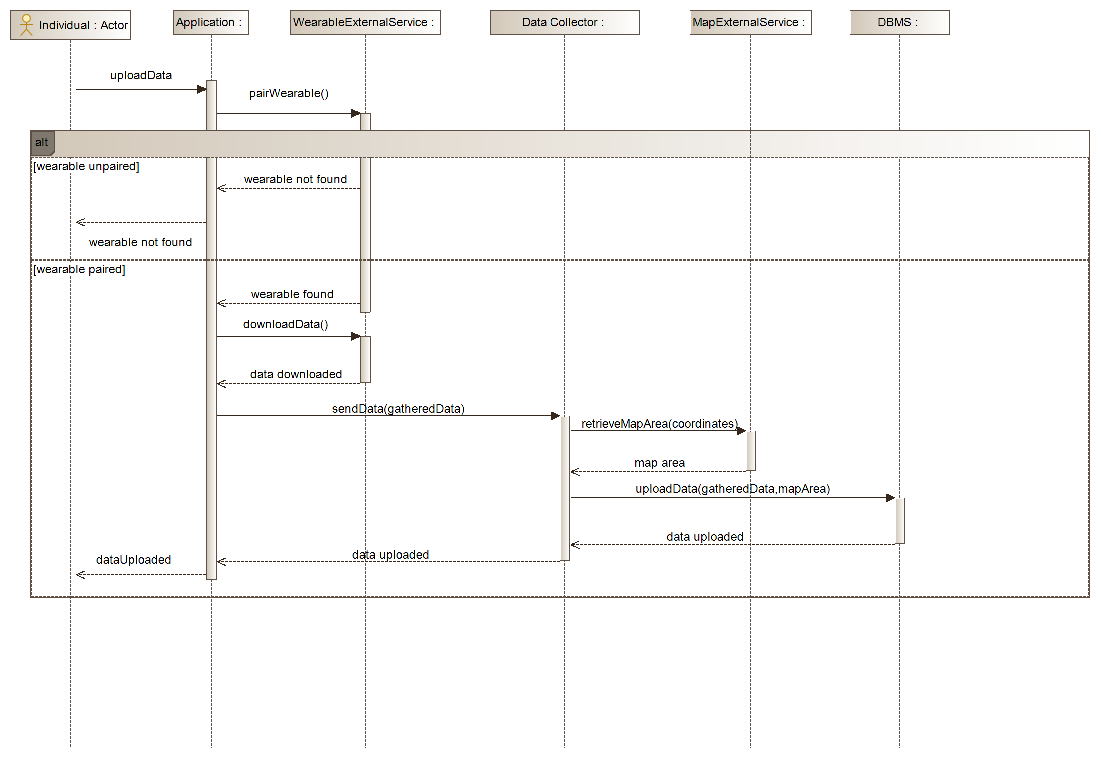
\includegraphics[width=\linewidth]{resources/uml/sequence/wearablePairing.png}
\end{figure}

\subsection{AutomatedSOS subscription}
\begin{figure}[h]
\centering
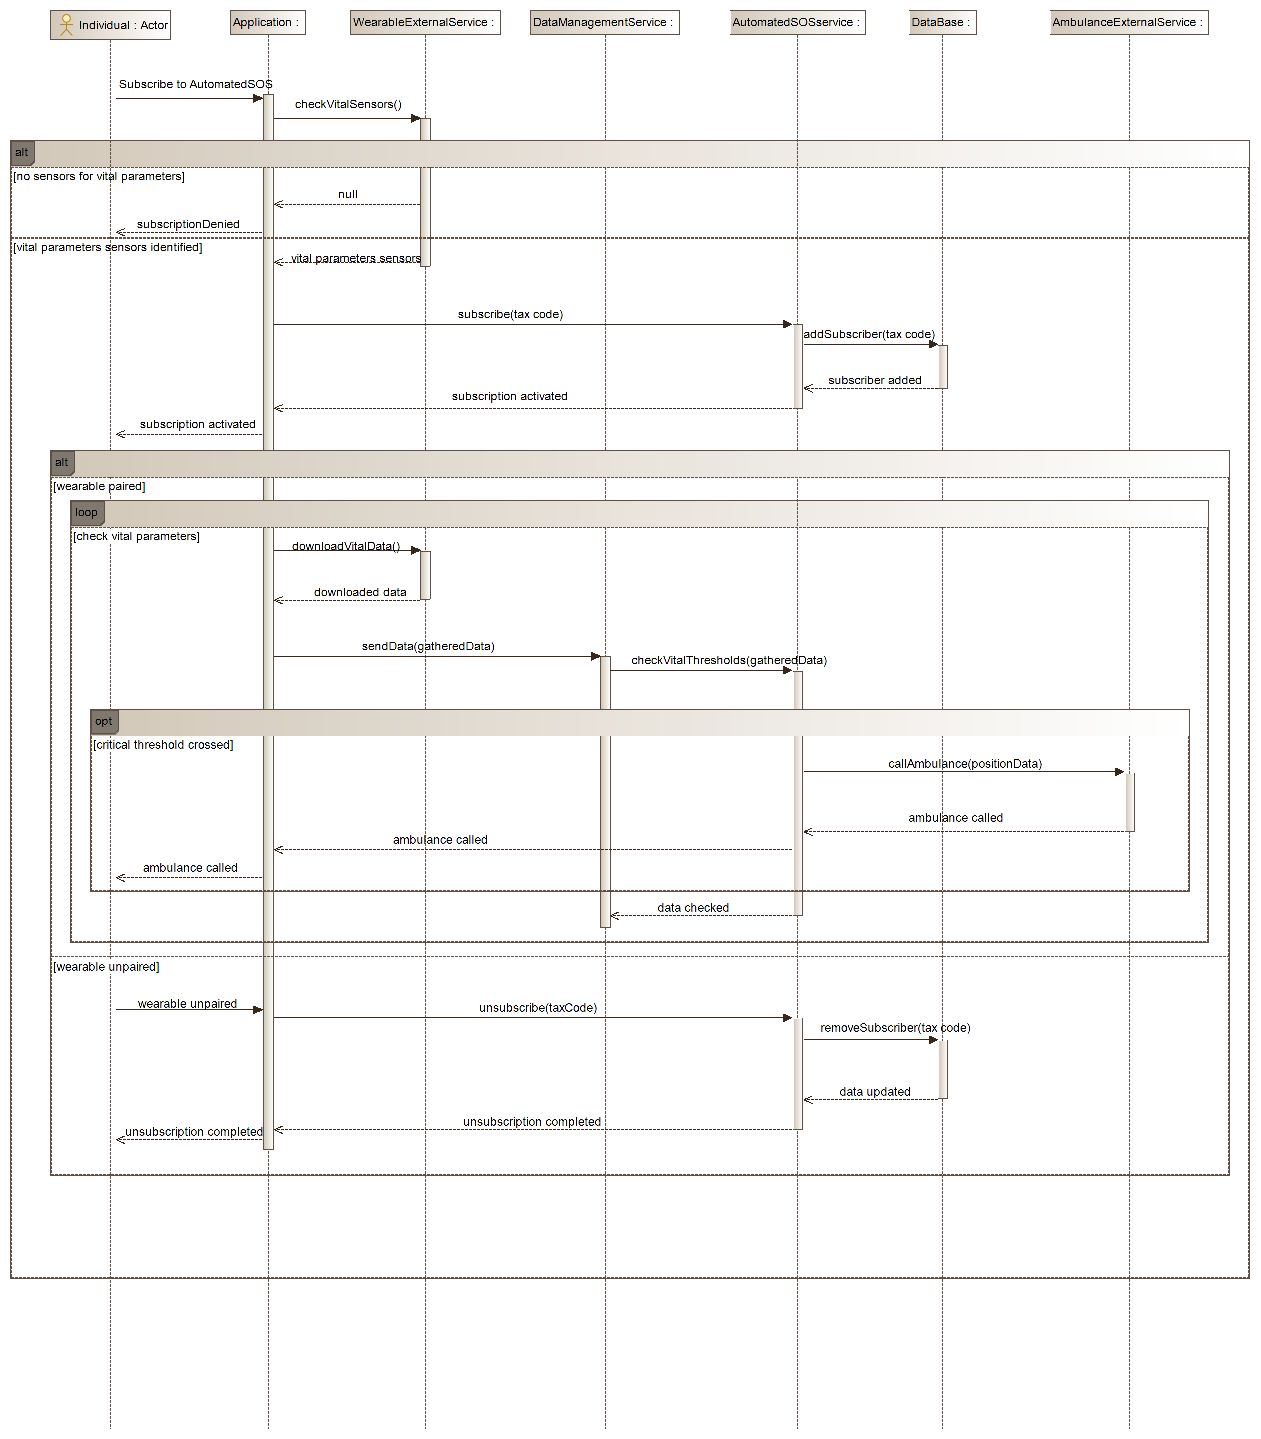
\includegraphics[width=\linewidth]{resources/uml/sequence/AutomatedSOS.png}
\end{figure}


\subsection{Group Data Request}
\begin{figure}[h]
\centering
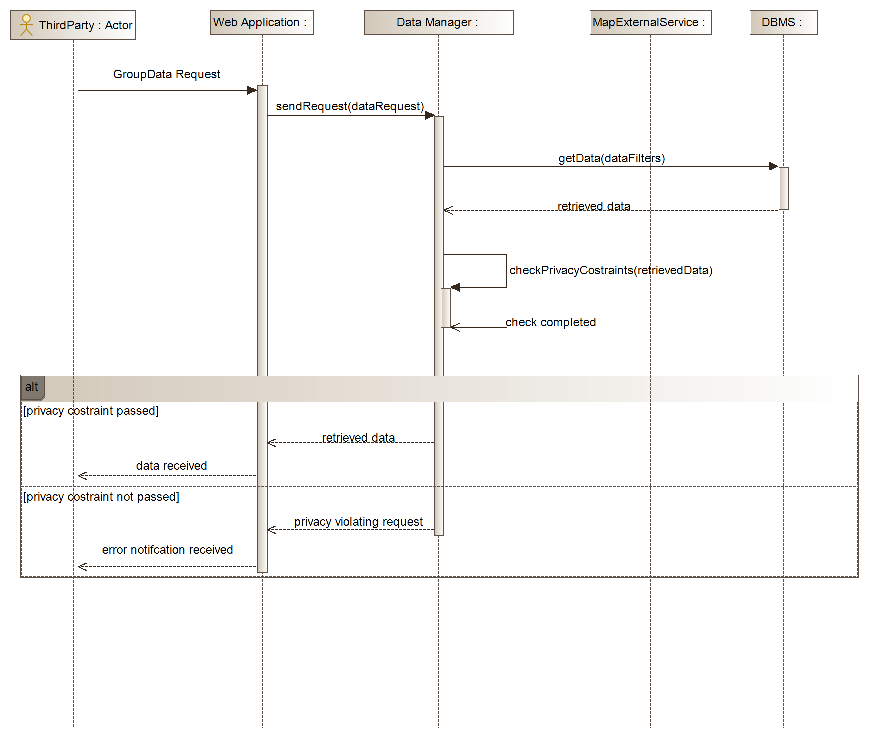
\includegraphics[width=\linewidth]{resources/uml/sequence/RequestGroupData.png}
\end{figure}

\subsection{Individual Data request}
\begin{figure}[h]
\centering
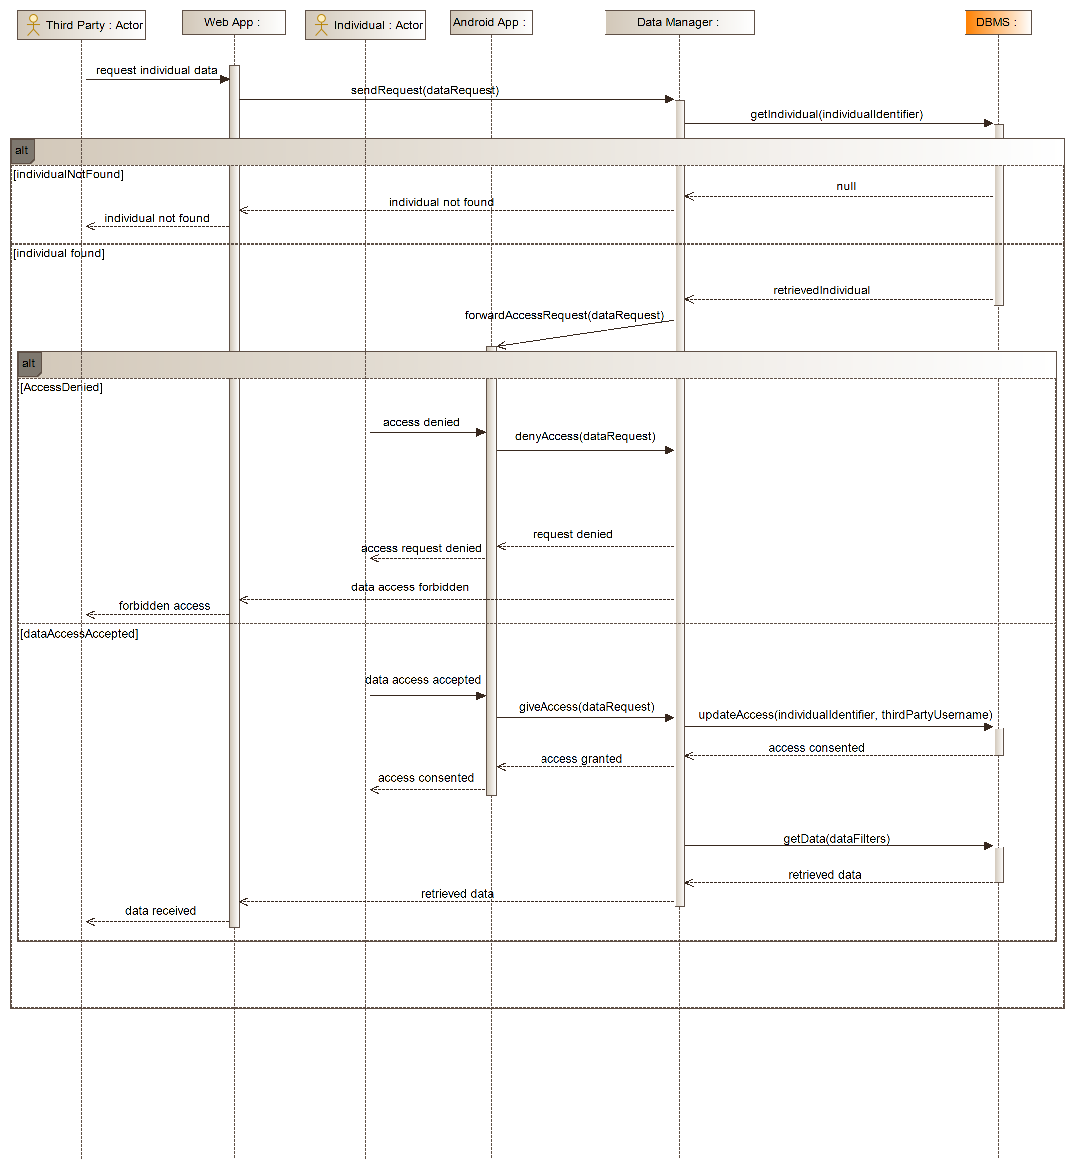
\includegraphics[width=\linewidth]{resources/uml/sequence/RequestIndividualData.png}
\end{figure}

\subsection{Data subscription}
\begin{figure}[h]
\centering
\includegraphics[width=\linewidth]{resources/uml/sequence/DataSubscription.png}
\end{figure}

















